\section{Daredevil y su astigmatismo}

Daredevil está muy preocupado con la situación de la salud en el país, ya que le dijeron que mientras más ciego esté,  más fila le toca hacer para reclamar los medicamentos para la ceguera. Dado que él no está seguro del porcentaje de miopía y astigmatismo que presenta, decide pedir una cita con el oftanmólogo. Sin embargo, se la dieron para septiembre. El punisher le dice entonces que la única forma de lograr la cita rápido, es armando un mierdero en la EPS, pero este se rehusa a armarlo, y mejor averigua en chat gpt ¿cuál es la formula para calcular el porcentaje de miopía y astigmatismo de una persona?. La IA le arroja la siguiente expresión:

\[ f(x) = \frac{A\times10^{-2}}{8} \cos \left(x - A\times10^{-3} \right) - x \]

Siendo $x \times 100\%$ el porcentaje de miopia y astigmatismo de la persona,
el cual se obtiene cuando se hace $f(x) = 0$, y $A$ corresponde a $510$.


\subsection{Ayude al Diablo (1 pt)}

Ayude  al Diablo a calcular su porcentaje de ceguera, usando $510$, y el
método de punto fijo con una tolerancia de 6 cifras significativas, y una
condición inicial $x_0 = 0$. Note que $g(x) = f(x) - x$.
Dé una respuesta al Diablo, y entregue la tabla solución en el formato visto en clase.

\begin{figure}[H]
    \centering
    \begin{subfigure}[b]{\textwidth}
        \centering
        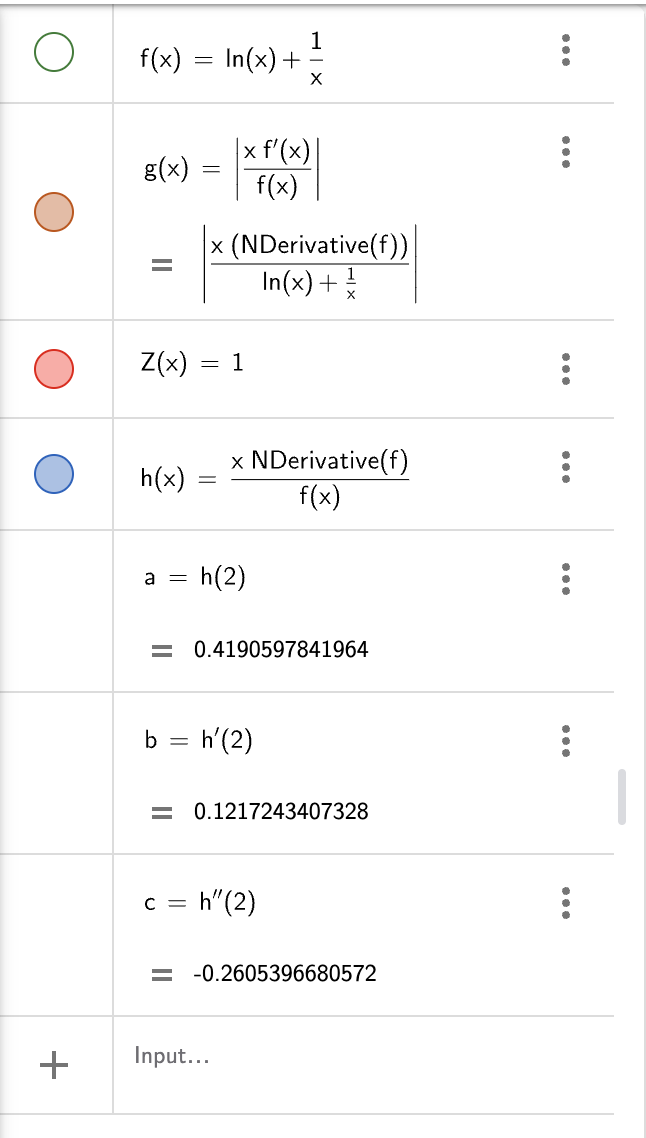
\includegraphics[width=0.4\textwidth]{Figures/0. General/1.2.png}
        \caption{Comprobación de valores $G(2)$, $G'(2)$ y $G''(2)$ en Geogebra}
        \label{fig: Comprobacion en Geogebra}
    \end{subfigure}
\end{figure}
